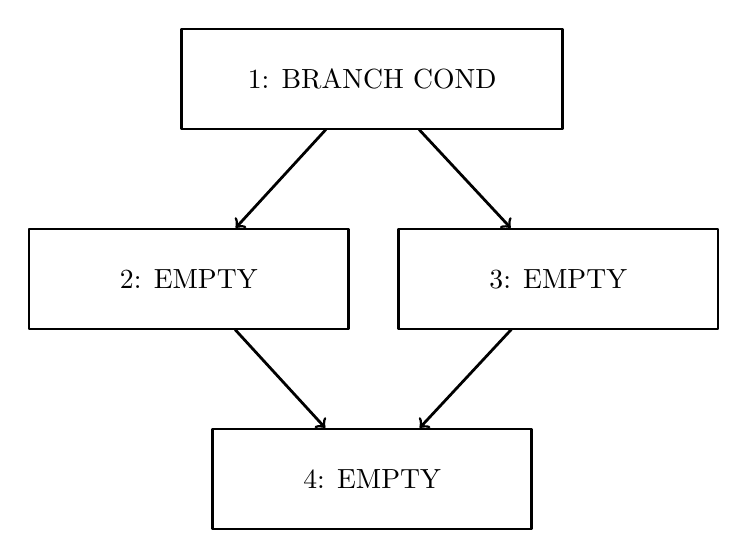
\begin{tikzpicture}[line join=bevel,]
\pgfsetlinewidth{1bp}
%%
\begin{scope}
\pgfsetstrokecolor{black}
\definecolor{strokecol}{rgb}{1.0,1.0,1.0};
\pgfsetstrokecolor{strokecol}
\definecolor{fillcol}{rgb}{1.0,1.0,1.0};
\pgfsetfillcolor{fillcol}
\filldraw (0.0bp,0.0bp) -- (0.0bp,180.0bp) -- (248.0bp,180.0bp) -- (248.0bp,0.0bp) -- cycle;
\end{scope}
\pgfsetcolor{black}
% Edge: 1 -> 2
\draw [->] (106.85bp,143.83bp) .. controls (99.089bp,135.37bp) and (89.72bp,125.15bp)  .. (74.379bp,108.41bp);
% Edge: 3 -> 4
\draw [->] (173.59bp,71.831bp) .. controls (165.72bp,63.369bp) and (156.21bp,53.149bp)  .. (140.63bp,36.413bp);
% Edge: 1 -> 3
\draw [->] (140.41bp,143.83bp) .. controls (148.28bp,135.37bp) and (157.79bp,125.15bp)  .. (173.37bp,108.41bp);
% Edge: 2 -> 4
\draw [->] (74.155bp,71.831bp) .. controls (81.911bp,63.369bp) and (91.28bp,53.149bp)  .. (106.62bp,36.413bp);
% Node: 1
\begin{scope}
\definecolor{strokecol}{rgb}{0.0,0.0,0.0};
\pgfsetstrokecolor{strokecol}
\draw (192.0bp,180.0bp) -- (55.0bp,180.0bp) -- (55.0bp,144.0bp) -- (192.0bp,144.0bp) -- cycle;
\draw (123.5bp,162.0bp) node {1: BRANCH COND};
\end{scope}
% Node: 3
\begin{scope}
\definecolor{strokecol}{rgb}{0.0,0.0,0.0};
\pgfsetstrokecolor{strokecol}
\draw (248.0bp,108.0bp) -- (133.0bp,108.0bp) -- (133.0bp,72.0bp) -- (248.0bp,72.0bp) -- cycle;
\draw (190.5bp,90.0bp) node {3: EMPTY};
\end{scope}
% Node: 2
\begin{scope}
\definecolor{strokecol}{rgb}{0.0,0.0,0.0};
\pgfsetstrokecolor{strokecol}
\draw (115.0bp,108.0bp) -- (0.0bp,108.0bp) -- (0.0bp,72.0bp) -- (115.0bp,72.0bp) -- cycle;
\draw (57.5bp,90.0bp) node {2: EMPTY};
\end{scope}
% Node: 4
\begin{scope}
\definecolor{strokecol}{rgb}{0.0,0.0,0.0};
\pgfsetstrokecolor{strokecol}
\draw (181.0bp,36.0bp) -- (66.0bp,36.0bp) -- (66.0bp,0.0bp) -- (181.0bp,0.0bp) -- cycle;
\draw (123.5bp,18.0bp) node {4: EMPTY};
\end{scope}
%
\end{tikzpicture}
